\section{Grid companies}
\label{app:grids}
\begin{figure}[H]
  \centering
  \caption{Grid companies in may 2019}
  \label{fig:elnetgraenser}
    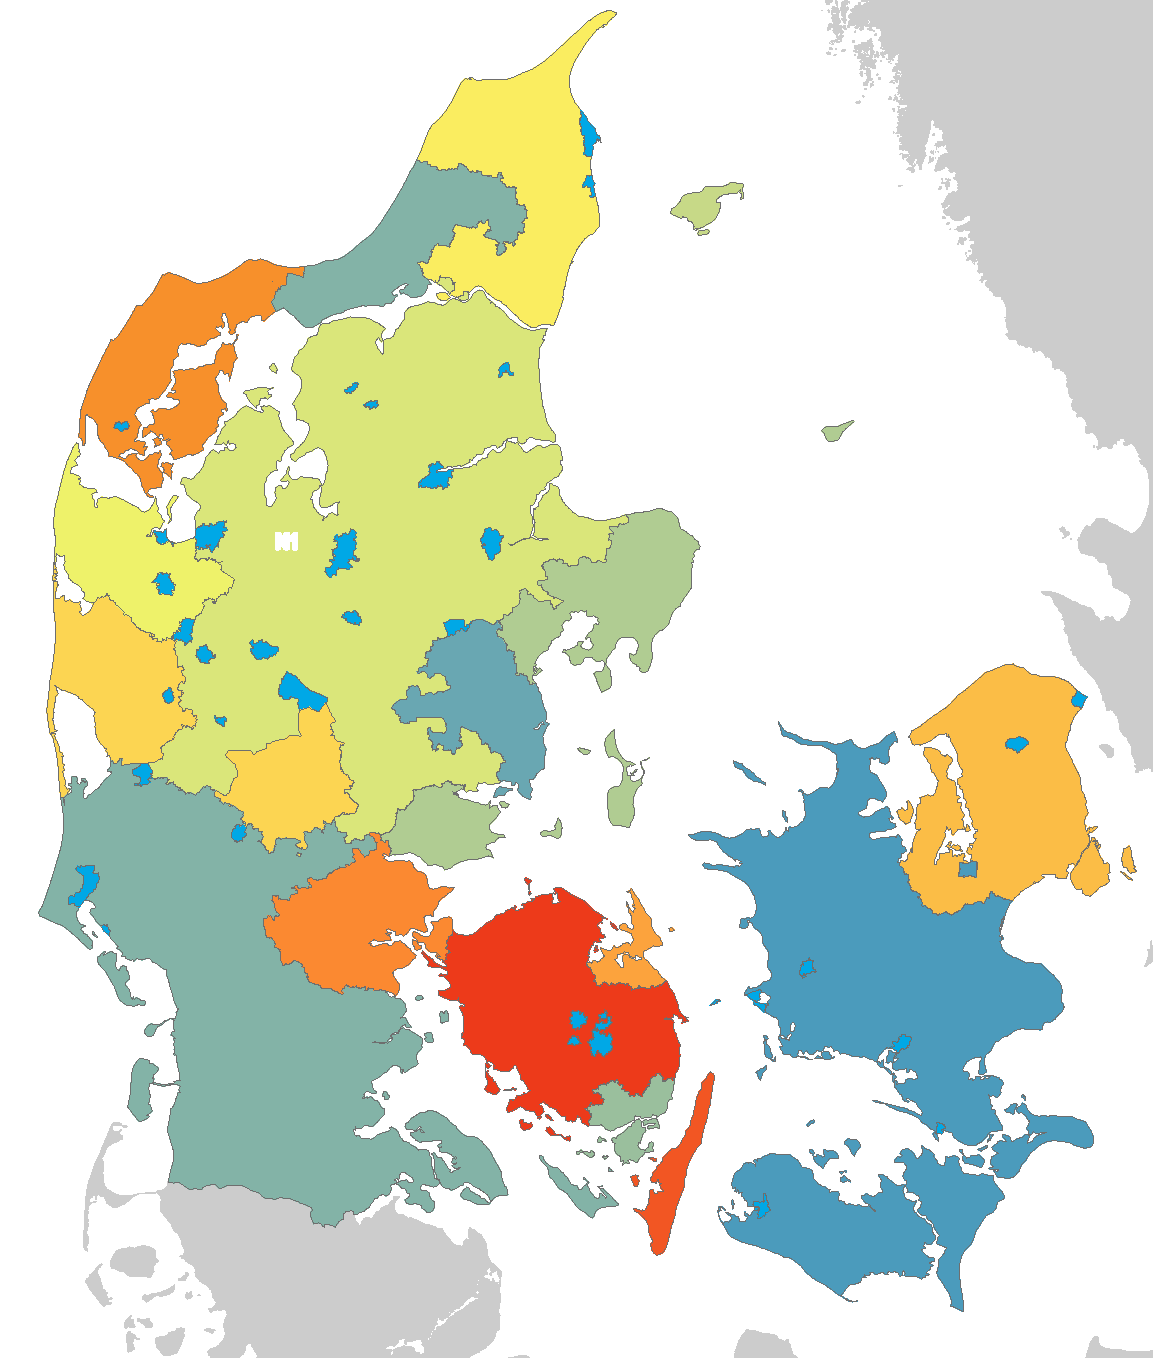
\includegraphics[width=.9 \textwidth]{03_figures/elnetgraenser_maj2019.pdf}
  \sourcecenter{Danish Energy Agency (Energistyrelsen).}
\end{figure}
\vspace{-1em}
\noindent
Mergers during 2016-2018:
\begin{itemize}[noitemsep]
  \item Nord Energi took over Taars by December 2017 and Hirtshals by January 2018.
  \item Læsø took over Hornum by October 2017.
  \item EnergiMidt merged with HEF, AKE, Bjerringbro, ELRO, EnergiMidt Vest, Borris, and Sdr. Felding by January 2018 and Nibe by April 2018, taking the name Eniig and later N1.
  \item Dinel was founded as a merge of Brabrand, Viby, GE, and Østjysk by April 17.
  \item SE took over VOS and Ærø by January 2018, later renaming to Evonet.
  \item RAH Net took over RAH Net 2 by December 2017 and MES Net by March 2018.
\end{itemize}
%To distinguish the grid name from the parent company Nyfors, NRGI, Energi Fyn, and SEAS-NVE has renamed to Evonet, Konstant, Vores Elnet, and Cerius respectively.
